\chapter{Relevant probability distributions}
\label{chap:probdistributions}

This appendix details the most important probability distributions employed in this thesis.  For each distribution, we provide its parameters, probability density or mass function (depending on whether the distribution has a discrete or continuous domain), mean and variance. 

\section*{Continuous uniform distribution}

\begin{description}
\item [Parameters: ] Continuous uniform distributions are described by two parameters $a$ and $b$ that define the range $[a,b]$ upon which the distribution is defined. 

\item [Density function: ] The density remains constant within $[a,b]$ and is $0$ outside this range:
\begin{equation}
P(x\,; a, b) = \begin{cases}
\frac{1}{b - a} & \text{for } x \in [a,b]  \\
0               & \text{otherwise}
\end{cases}
\end{equation} 
\item [Mean: ] The mean of a continuous uniform distribution is simply equal to \ $\dfrac{a+b}{2}$

\item [Variance: ] The distribution variance is \ $\dfrac{(b-a)^2}{12}$
\end{description}

\begin{figure}[h]
\centering
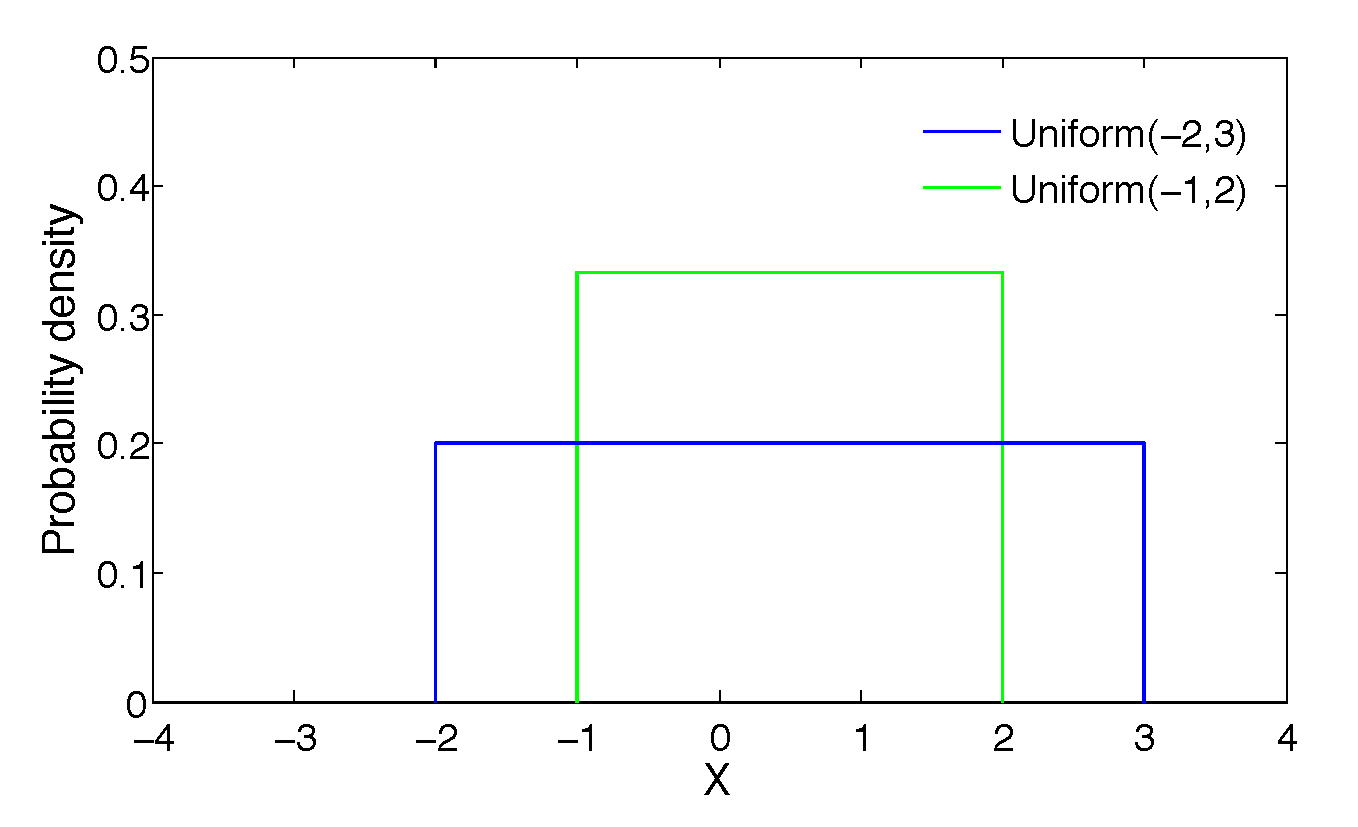
\includegraphics[scale=0.40]{imgs/uniform-appendix.pdf}
\caption{Probability density functions for two continuous uniform distributions.} 
\label{fig:uniform-appendix}
\end{figure}

\section*{Discrete uniform distribution}

\begin{description}
\item [Parameters: ] Discrete uniform distributions are also described by two parameters $a$ and $b$, but are here constrained to integer values. The number $n$ of values in the distribution is $b-a+1$. 

\item [Probability mass function: ] The probability mass function is defined as:
\begin{equation}
P(X\!=\!i\,; a, b) = \begin{cases}
\frac{1}{n} & \text{for } i \in \mathcal{Z} \text{ and } \in [a,b]  \\
0               & \text{otherwise}
\end{cases}
\end{equation} 
\item [Mean: ] The mean of a discrete uniform distribution is also \  $\dfrac{a+b}{2}$

\item [Variance: ] The distribution variance is \ $\dfrac{(n^2 -1)}{12}$
\end{description}

\begin{figure}[h]
\centering
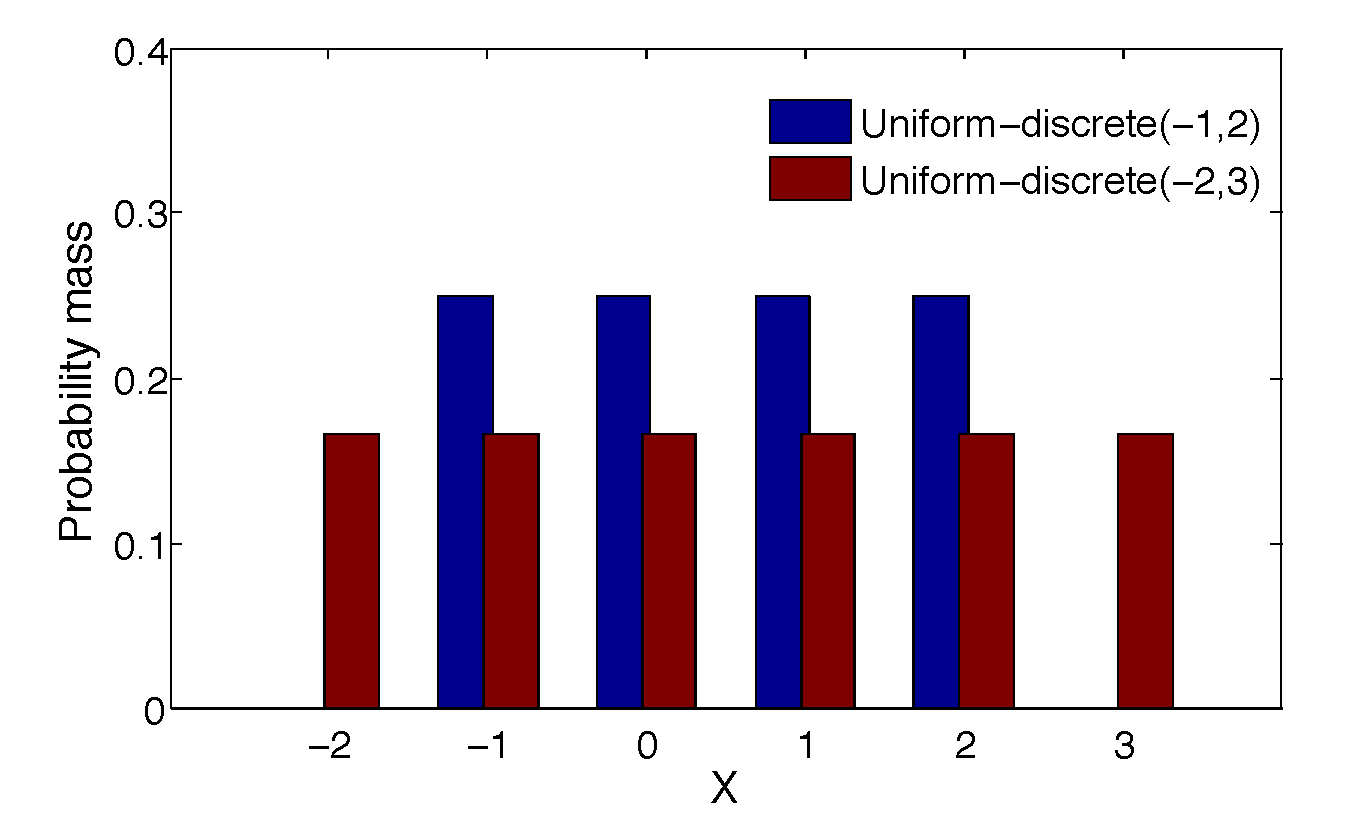
\includegraphics[scale=0.40]{imgs/uniformd-appendix.pdf}
\caption{Probability mass functions for two discrete uniform distributions.} 
\label{fig:uniformd-appendix}
\end{figure}

\section*{Categorical distribution}

A categorical distribution describe the result of a random event that can take on one of $K$ possible (and mutually exclusive) outcomes.

\begin{description}
\item [Parameters: ] A categorical distributions on $K$ outcomes is defined by $K$ parameters $p_1, \dots, p_K$ representing the probabilities of each outcome.

\item [Probability mass function: ] The probability mass function is simply defined as:
\begin{equation}
P(X=i\,; p_1, \dots, p_K) = p_i
\end{equation} 
\end{description}

The mean and variance of categorical distributions are only defined when the outcomes have a numerical range.  The mean is in this case equal to $\mu = \sum_{i=1}^{K} i\, p_i$, while the variance corresponds to $\sigma^2 = \sum_{i=1}^K (p_i\, i^2) - \mu^2$.

\begin{figure}[h]
\centering
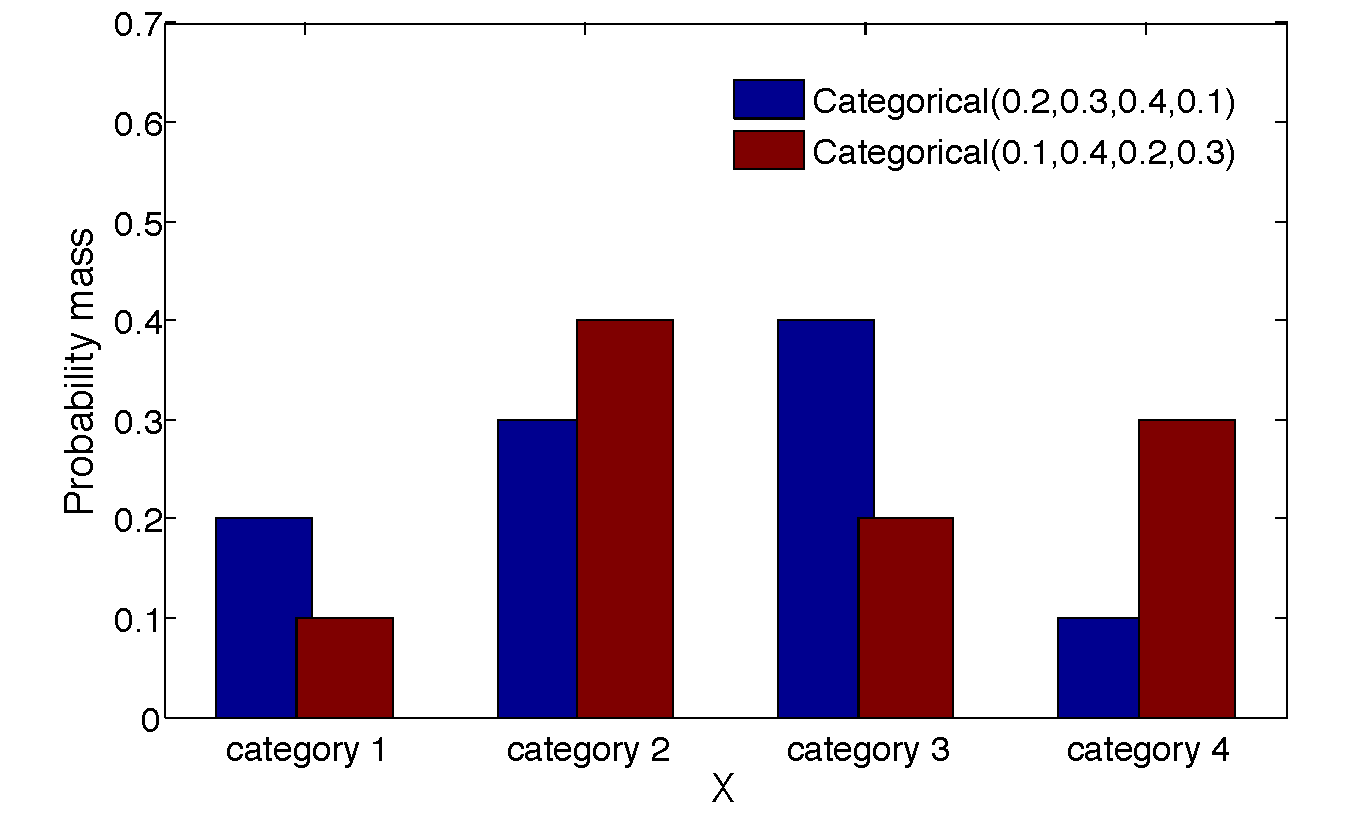
\includegraphics[scale=0.40]{imgs/categorical_appendix.pdf}
\caption{Probability mass functions for two categorical distributions.} 
\label{fig:categorical-appendix}
\end{figure}

\section*{Multinomial distribution}

Given the repetition of $n$ independent trials where each trial leads to one of $K$ possible outcomes (described by a categorical distribution), the multinomial distribution gives the probability of a particular combination of numbers of outcomes for the various categories. 

\begin{description}
\item [Parameters: ] Multinomial distributions are parametrised with $K$ probability values $p_1, \dots, p_K$ expressing the likelihood of each outcome, and an integer $n$ denoting the number of trials.

\item [Probability mass function: ] For $n$ trials,  the probability of having $x_1$ outcomes for category 1, $x_2$ outcomes for category 2, \dots, and $x_K$ outcomes for category $K$ is:
\begin{align}
P(X_1 = x_1,\dots, X_K = x_K)  = \begin{cases} { \displaystyle {n! \over x_1!\dots x_K!}\ p_1^{x_1} \dots p_K^{x_K}} \quad &
\mbox{when } \sum_{i=1}^K x_i=n \\
0 & \mbox{otherwise} \end{cases}
\end{align} 
\item [Mean: ] The expected number of outcomes for a category $i$ is \ $ n p_i$.

\item [Variance: ] The variance on the number of outcomes for a category $i$ is \ $n  p_i (1-p_i)$.
\end{description}

\begin{figure}[h!]
\centering
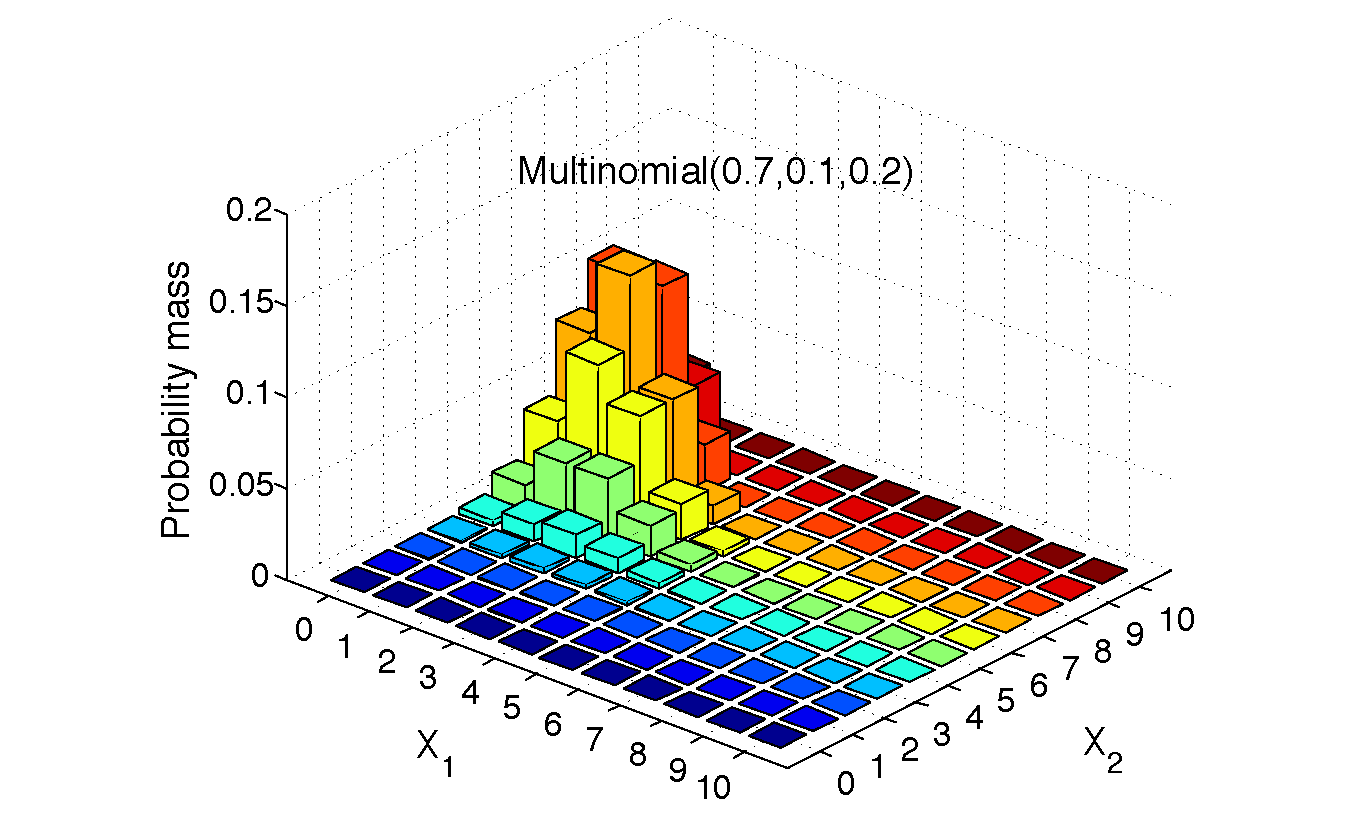
\includegraphics[scale=0.40]{imgs/multinomial_appendix.pdf}
\caption{Probability mass function for a multinomial distribution.} 
\label{fig:multinomial-appendix}
\end{figure}

The binomial distribution is a special case of multinomial with only two categories.  The binomial distribution expresses the number of successes associated with the repetition of $n$ Bernoulli trials with a specific probability of success. 

\section*{Normal distribution}

The normal distribution (also called the Gaussian distribution or the bell curve) is the most well known probability distribution in the continuous domain. The central limit theorem states that, under mild conditions, the mean of many random variables drawn independently from the same (arbitrary) distribution is distributed according to a normal distribution in the large sample limit.   


\begin{description}
\item [Parameters: ] A normal distribution is encoded by two parameters: the mean $\mu$ and  variance $\sigma^2$. 

\item [Probability density function: ] The density function of a normal distribution is defined as:
\begin{equation}
P(x \,; \mu,\sigma^2) = \frac{1}{\sqrt{2\pi\sigma^2}}\ \operatorname{exp}\left\{-\frac{\left(x-\mu\right)^2}{2\sigma^2}\right\}
\end{equation}
\item [Mean: ] The mean of the normal distribution corresponds to $\mu$.

\item [Variance: ] The variance of the distribution is $\sigma^2$.

\end{description}

\begin{figure}[h!]
\centering
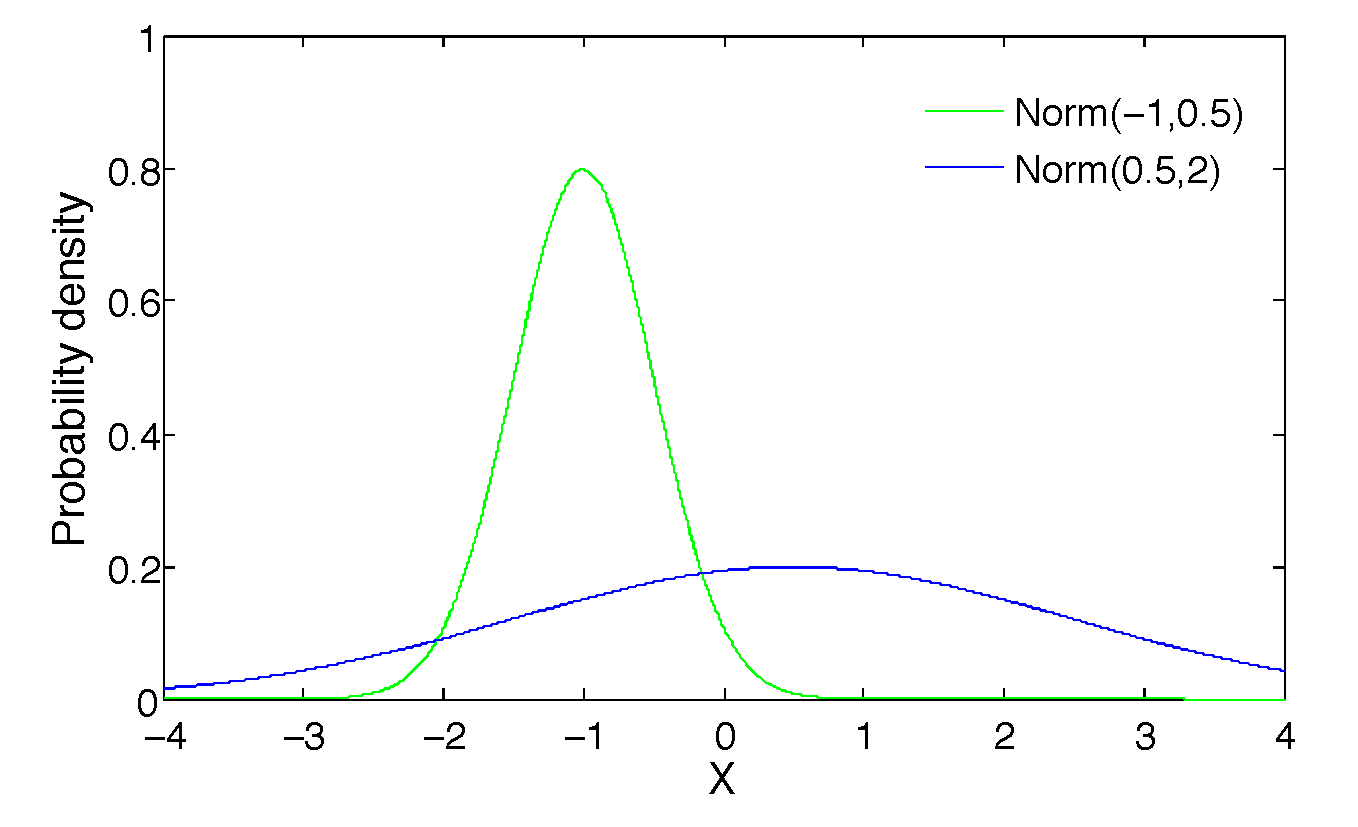
\includegraphics[scale=0.40]{imgs/norm_appendix.pdf}
\caption{Probability density functions for two normal distributions.} 
\label{fig:norm-appendix}
\end{figure}


Multivariate normal distributions can be used to generalise one-dimensional normal distributions to higher dimensions. Multivariate normal distributions of dimensions $K$ are parametrised by a $K$-dimensional mean vector $\boldsymbol\mu$ and a $(K \times K)$-dimensional covariance matrix $\boldsymbol\Sigma$. 

\section*{Dirichlet distribution}

A Dirichlet is a continuous, multivariate probability distribution that is often used to describe the parameters of categorical or multinomial distributions.  The Dirichlet distribution is indeed the conjugate prior of these distributions. 

\begin{description}
\item [Parameters: ] A Dirichlet distribution of dimension $K$ is encoded by $K$ parameters $\boldsymbol\alpha = \alpha_1, \dots, \alpha_K$. 

\item [Probability density function: ] The density function of a Dirichlet distribution is defined as:
\begin{align}
P(x_1, \dots, x_K\,; \boldsymbol\alpha) = \frac{1}{\mathrm{B}(\boldsymbol\alpha)} \prod_{i=1}^K x_i^{\alpha_i - 1} \ \ \ \text{with } \mathrm{B}(\boldsymbol\alpha) = \frac{\prod_{i=1}^K \Gamma(\alpha_i)}{\Gamma\bigl(\sum_{i=1}^k \alpha_i\bigr)}
\end{align}
in which $ \mathrm{B}(\boldsymbol\alpha)$ is a normalisation factor and $\Gamma$ is the gamma function $\Gamma(z) = \int_0^\infty  t^{z-1} e^{-t}\,{\rm d}t$. 

\item [Mean: ] The mean of the $i$-th component of the Dirichlet distribution is $\dfrac{\alpha_i}{\sum_k \alpha_k}$.

\item [Variance: ] The variance of the $i$-th component is $\dfrac{\alpha_i (\alpha_0-\alpha_i)}{\alpha_0^2 (\alpha_0+1)} \text{ with } \alpha_0 = \sum_{i=1}^K\alpha_i$.

\end{description}

\begin{figure}[h!]
\centering
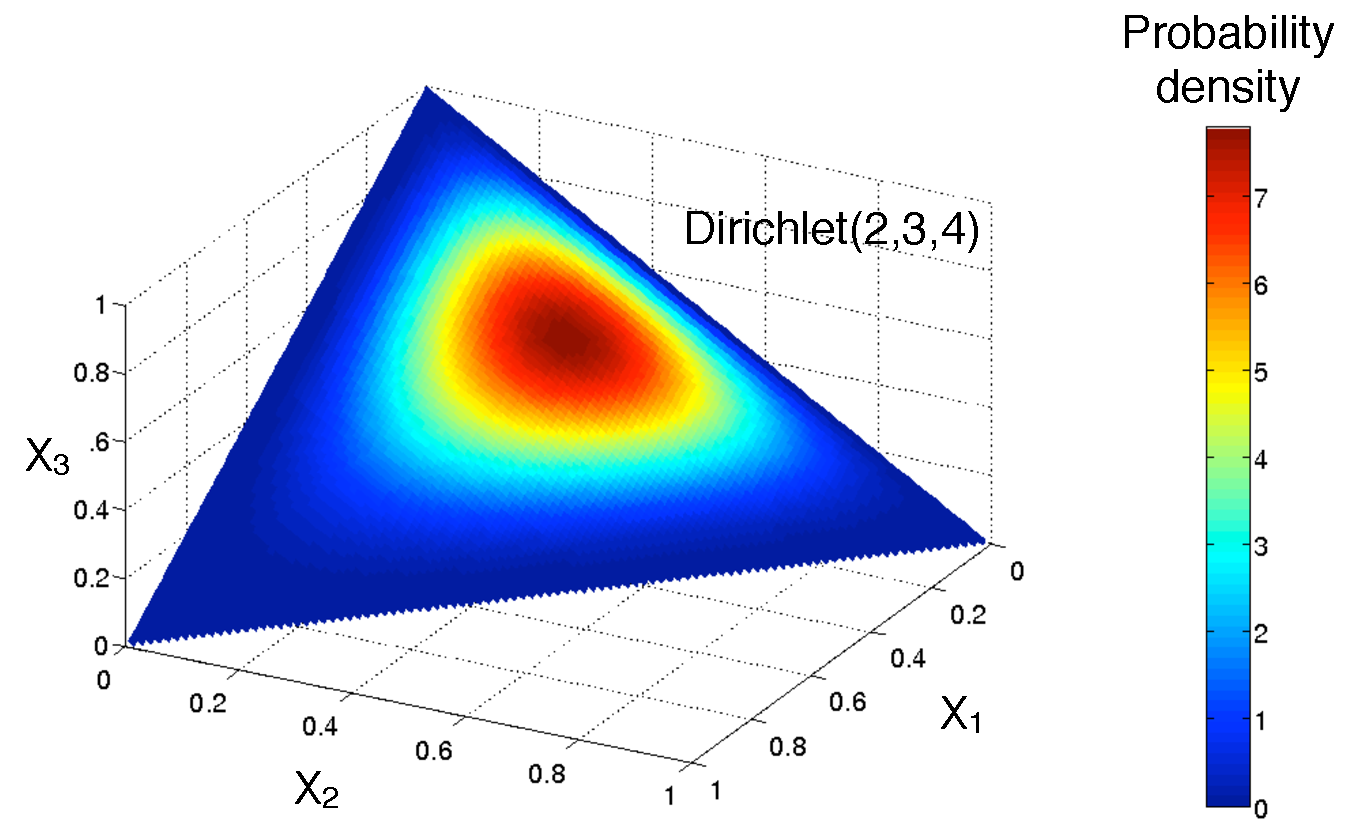
\includegraphics[scale=0.40]{imgs/dirichlet_appendix.pdf}
\caption{Probability density function for a three-dimensional Dirichlet distribution.} 
\label{fig:dirichlet-appendix}
\end{figure}



\section*{Geometric distribution}

A geometric distribution is a discrete probability distribution that describes the number of Bernoulli trials required to get one success. 

\begin{description}
\item [Parameters: ] Geometric distributions are defined by the parameter $p$ that encodes the probability of success for each Bernoulli trial. 

\item [Probability mass function: ] Given a constant probability $p$ of success for each trial, the probability that the $k$th trial will result in the first success is:
\begin{equation}
P(X = k) = (1-p)^{k-1}\,p\,
\end{equation}

\item [Mean: ] The expected number of trials needed to get one success is $\frac{1}{p}$.

\item [Variance: ] The variance on the numbers of trials to get the first success is $\frac{1-p}{p^2}$. 

\end{description}


\begin{figure}[t]
\centering
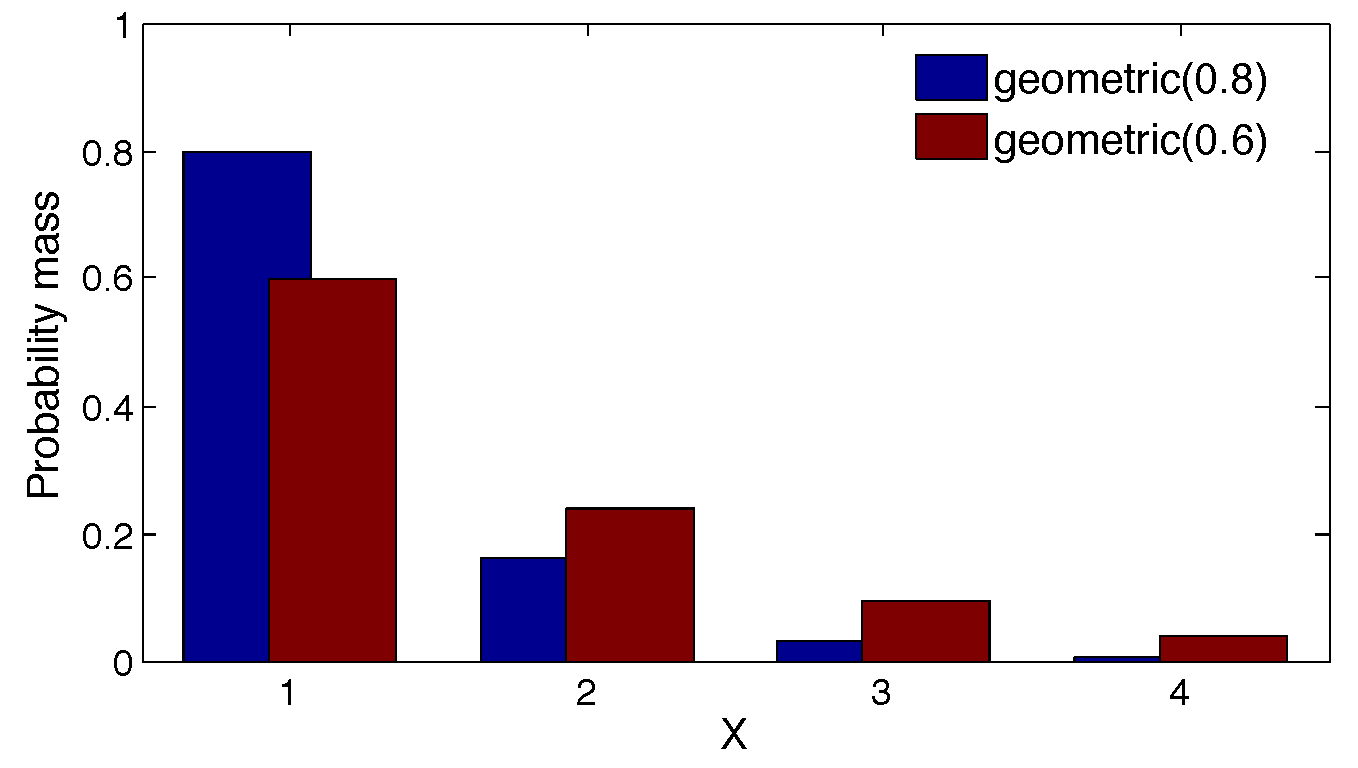
\includegraphics[scale=0.40]{imgs/geometric_appendix.pdf}  \vspace{-2mm}
\caption{Probability mass function for two geometric distributions. } 
\label{fig:geometric-appendix}
\end{figure}



\section*{Kernel distribution}

Distributions can also be defined in a non-parametric manner using kernel density estimation (KDE).  Such distributions are constructed on the basis of a set of sample points $x_1, \dots, x_n$.

\begin{description}
\item [Parameters: ] A kernel distribution is fully defined by its sample points, the kernel function $K(\cdot)$, and the smoothing bandwidth $h$.  Multiple kernels are possible but a common choice is the Gaussian distribution.

\item [Probability density function: ] The kernel density estimator for the points $x_1, \dots, x_n$ is: 
\begin{align}
P(x) = \frac{1}{nh} \sum_{i=1}^n K\Big(\frac{x-x_i}{h}\Big)
\end{align}
\item [Mean: ] The mean of kernel density estimate is the average of the sample points: $\dfrac{\sum_{i=1}^n x_i}{n}$.

\item [Variance: ] The variance of the estimate is $\sigma^2 + h^2 \kappa$, where $\sigma^2$ is the variance of the sample points and $\kappa$ corresponds to the variance of the kernel. 

\end{description}

\begin{figure}[h]
\centering
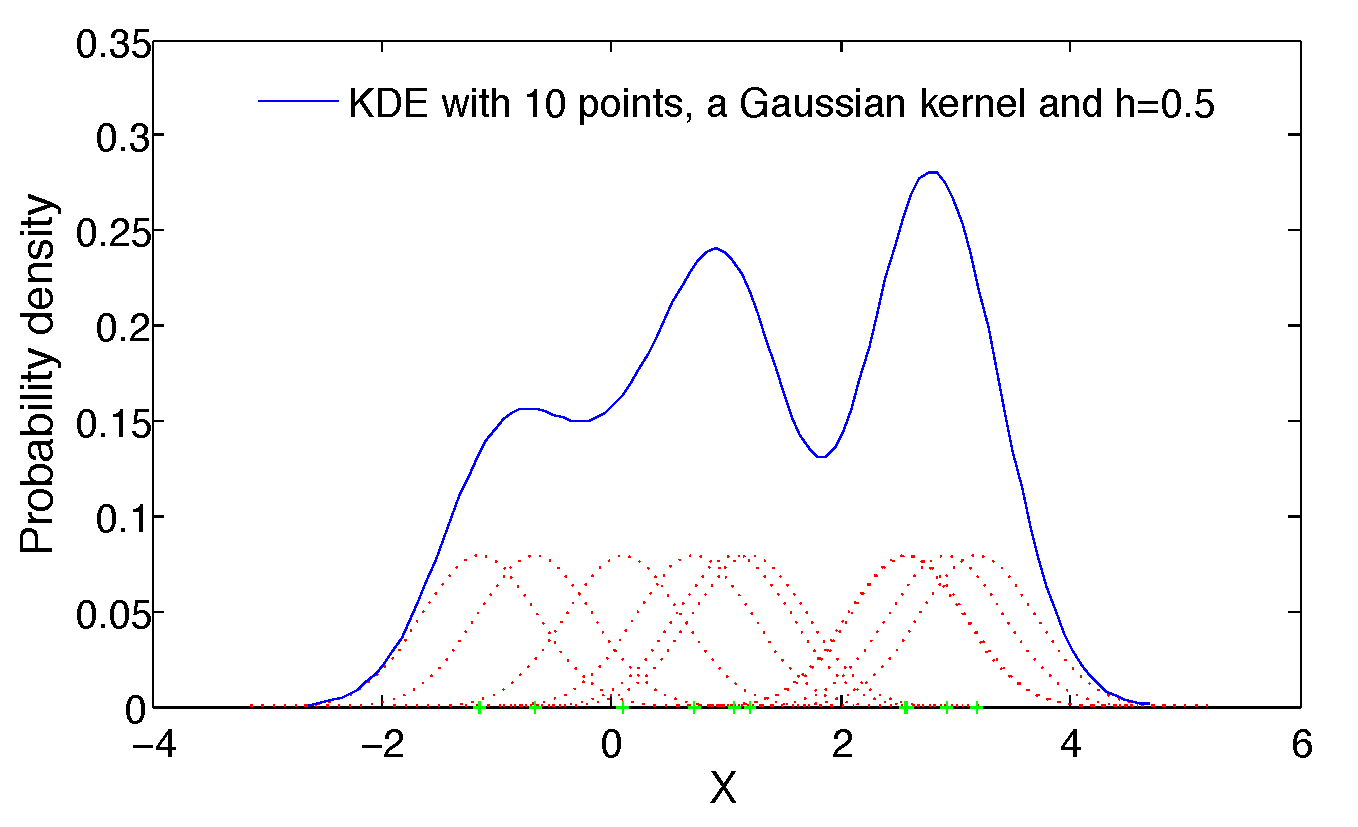
\includegraphics[scale=0.40]{imgs/kde_appendix.pdf} \vspace{-2mm}
\caption{Probability density function for a kernel density estimate with ten points. The Gaussian distributions making up the estimate are shown with red dashed lines. } 
\label{fig:kde-appendix}
\end{figure}


